\section{The Standard Model of Particle Physics}

The Standard Model \cite{Spiesberger:2000ks} is an effective description of all known fundamental particles.  Despite this criticism, the Standard Model provides a valid framework for the description of Nature, from microscopic scales up to cosmological distances.The Standard Model consists of three components.

\subsection{Matter}

The first component states that the basic constituents of matter are leptons and quarks which are realized in three families of identical structure. The entire ensemble of these constituents has been identified experimentally. Table \ref{table:fermions} shows all the fermions of the Standard Model and their charges, arranged in the three families.

	\begin{figure}[tbh!]
		\begin{center}
			
			\begin{tabular}{ | c | c | c | c | c |}
				\hline
				& 1st Generation & 2 Generation & 3rd Generation & charge \\ \hline \hline
				& & & & \\
				leptons & $\left( \begin{array}{c} \nu_{e} \\ e \end{array} \right)_{L}$ & $\left( \begin{array}{c} \nu_{\mu} \\ \mu \end{array} \right)_{L}$ & $\left( \begin{array}{c} \nu_{\tau} \\ \tau \end{array} \right)_{L}$ & \begin{tabular}{@{}c@{}}weak \\ weak, electromagnetic\end{tabular} \\
				& & & & \\
				 & $e_{R}$& $\mu_{R}$& $\tau_{R}$& electromagnetic\\ 
				 & & & & \\
				 \hline
				 & & & & \\
				leptons & $\left( \begin{array}{c} u \\ d \end{array} \right)_{L}$ & $\left( \begin{array}{c} c \\ s \end{array} \right)_{L}$ & $\left( \begin{array}{c} t \\ b \end{array} \right)_{L}$ & weak, electromagnetic, strong \\
				& & & & \\
				& $u_{R}, d_{R}$& $c_{R}, s_{R}$& $t_{R}, b_{R}$& electromagnetic, strong\\
				& & & & \\ 
				\hline
				\hline
			\end{tabular}
			\caption{Fermions of the Standard Model and their charges, arranged in the three generations. Only the left-handed fermions interact weakly and are arranged in doublets. The right-handed fermions are singlets. The right-handed neutrinos are not present in this table, as they do not interact with one of the forces of the Standard Model.}
			\label{table:fermions}
		\end{center}
	\end{figure}
	
	\begin{figure}[tbh!]
		\centering
		\begin{tabular}{cc}
			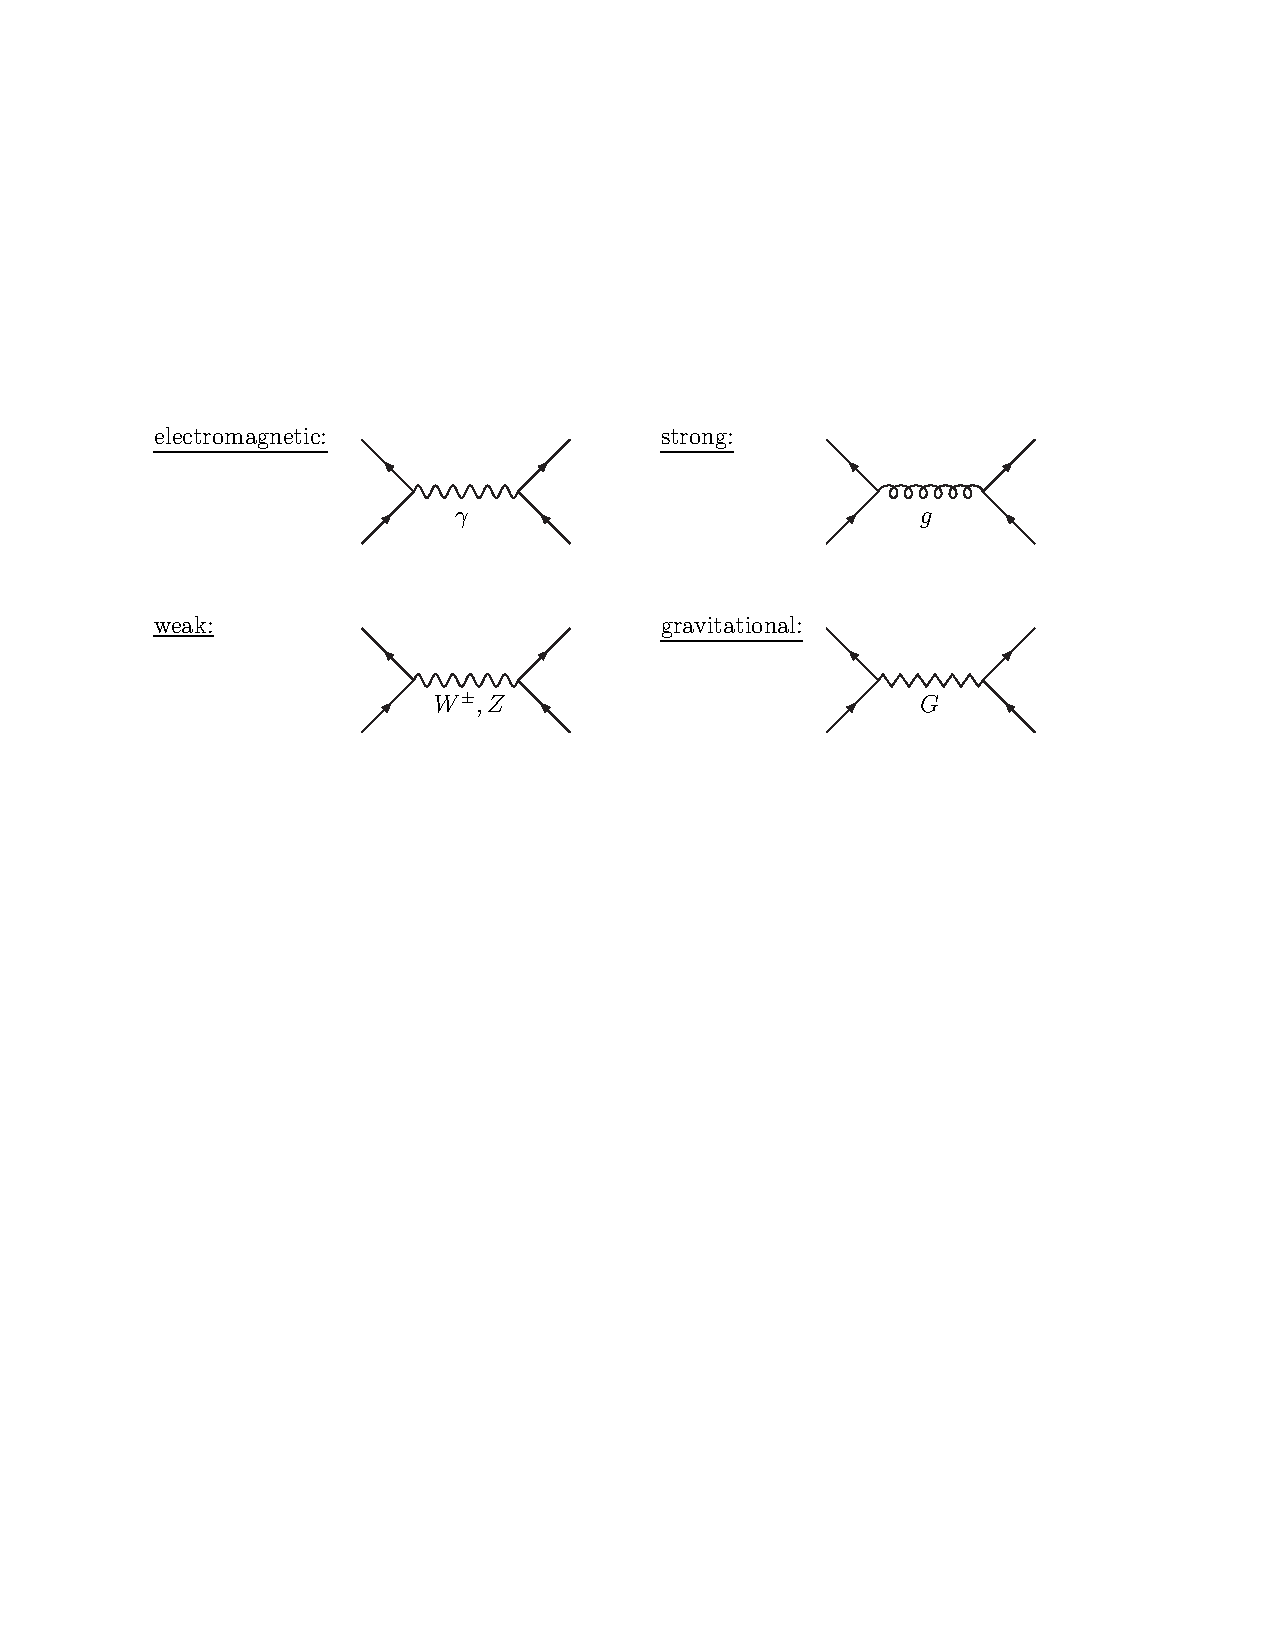
\includegraphics[width=0.75\textwidth]{theory/pics/SM_forces.pdf}
		\end{tabular}
		\caption{The four fundamental forces in nature as described by the Standard Model.}
		\label{fig:SM_forces}
	\end{figure}

\subsection{Interactions}

The interactions are mediated by bosons. They are the quanta of the gauge fields, and couple to the corresponding charges. The interactions are described by symmetry transformations U of the group SU(n). They are unitary (UU† = 1) and special (det(U) = 1). An operator


-----------------------------
	
The second component are the four different forces acting between the leptons and quarks. The electromagnetic and weak forces are unified in the Standard Model. The fields associated with these forces, as well as the fields associated with the strong force, are spin-1 fields, describing the photon \ensuremath{\gamma}, the electroweak gauge bosons \W and \Z, and the gluons g. The interactions of the force fields with the fermionic constituents of matter as well as their self-interactions are described by Abelian and non-Abelian \ensuremath{SU(3) \times SU(2) \times U(1)} gauge theories. The experimental exploration of these fundamental gauge symmetries is far advanced in the sector of lepton/quark-gauge boson interactions, yet much less is known so far from experiment about the self-interactions of the force fields. The gravitational interaction is mediated by a spin-2 field, describing the graviton G, with a character quite different from spin-1 gauge fields. The gravity sector is attached ad hoc to the other sectors of the Standard Model, not properly formulated yet as a quantum phenomenon. Figure \ref{fig:SM_forces} shows the four fundamental forces in nature as described by the Standard Model.



\begin{figure}[tbh!]
	\centering
	\begin{tabular}{cc}
		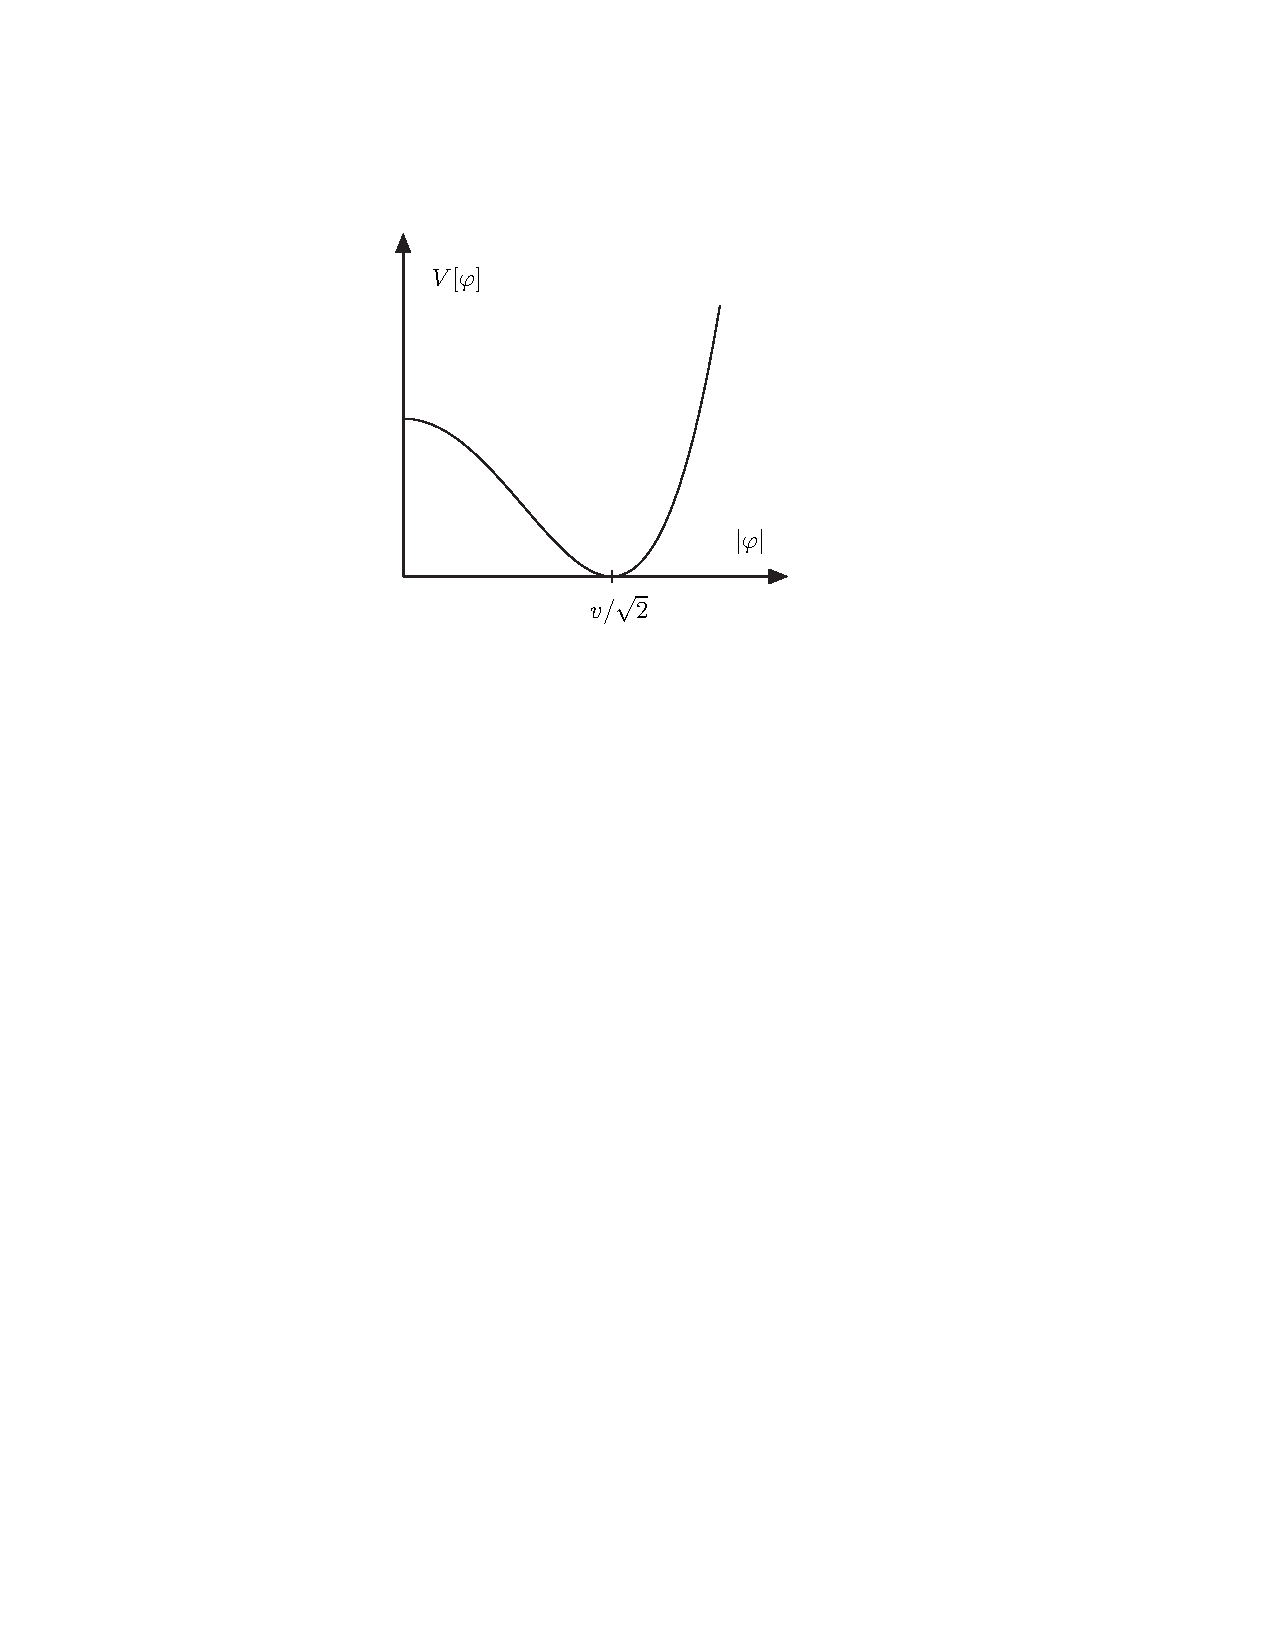
\includegraphics[width=0.75\textwidth]{theory/pics/higgs_potential.pdf}
	\end{tabular}
	\caption{The Higgs potential of the Standard Model.}
	\label{fig:higgs_potential}
\end{figure}


\subsection{The Higgs Mechanism}
Even though the Electroweak Unification lead to the successful discovery of the W and Z bosons this theory is formulated round massless particles. An elegant way to circumvent the problem is 
Riprendiamo il modello del Capitolo precedente ma promuoviamo la simmetria per trasformazioni di fase globale ad una simmetria per trasformazioni di fase dipendenti dal punto. Questo richiede, oltre al campo scalare complesso di partenza, l’ introduzione di un campo vettoriale Aμ analogo al campo elettromagntico, come discusso nel Cap. 3. La lagrangiana risultante `e:
 L = (Dμφ)† Dμφ − V (φ) − 1FμνFμν 4
 V(φ)=μ2φ†φ+λ(φ†φ)2 −εφ† −ε∗φ 
 Dμ = ∂μ − ieAμ
Fμν =∂νAμ−∂μAν
 Nel limite ε → 0, L `e invariante sotto le trasformazioni di gauge:
 φ(x) → eiα(x)φ(x); φ(x)† → e−iα(x)φ(x)†;
Aμ → Aμ + 1∂μα(x) e
(5.50)
(5.51) (5.52)
  dove α(x) `e una funzione reale arbitraria di x ed e una nuova costante di accoppiamento, che coincide con la carica elettrica se identifichiamo Aμ con il campo elettromagnetico. Come prima deve essere λ > 0, per ottenere una teoria stabile, ma μ2 pu`o avere entrambi i segni.
1. μ2 > 0. La configurazione di minima energia corrisponde a φ = 0, Aμ = 0. Se quantizziamo φ ed Aμ otteniamo una teoria con:
• una particella carica e la sua antiparticella, entrambe con massa μ ̸= 0;
• una particella di spin 1 e massa nulla (due stati di polarizzazione) in tutto simile al fotone;
Per λ ed e sufficientemente piccoli, la lagrangiana descrive le interazioni di particelle scalari con il campo elettromagnetico (elettrodinamica scalare, costante di accoppiamento e) e le loro autointerazioni (costante di accoppiamento λ).
La configurazione di minima energia si ottiene per Aμ = 0, per minimizzare l’ energia elettrostatica, quindi ricadiamo nel caso del modello di Goldstone, per cui (con ε → 0, reale):
  ̄  ̄  −μ2 V(φ)=min: φ=η= 2λ +O(ε)
Per studiare le fluttuazioni intorno alla configurazione di minimo, poniamo di nuovo: σ1(x) + iσ2(x)
e sviluppiamo la lagrangiana in (5.50). Lo spettro di massa delle particelle associate si ottiene come prima dai termini quadratici nei campi σi e Aμ. Prima di considerare questi termini, tuttavia, notiamo che sotto le trasformazioni (5.52) con α infinitesimo, il campo φ trasforma come:
  φ=η+ √2
(5.53)
(5.54)
    ovvero:
σ1(x) + iσ2(x)
φ → φ + iαφ = η + √2 + iηα(x) (5.55)
σ1(x) → σ1′ (x) = σ1(x); σ2(x) → σ2′ (x) = σ2(x) + √2ηα(x) (5.56)
 
dove abbiamo trattato sia le σi sia α come grandezze del primo ordine ed abbiamo trascura- to termini che sono almeno del secondo ordine. Naturalmente, allo stesso tempo dobbiamo trasformare Aμ secondo la (5.52).
Il campo σ2 si trasforma in modo non omogeneo per l’ aggiunta di un termine proporzionale ad α ma, a differenza del caso globale, il termine aggiuntivo `e una funzione di x di cui possiamo disporre a nostro piacimento. In particolare, dati i campi σi(x) ed Aμ(x), possiamo scegliere:
  in modo tale da avere:
σ2(x)
α(x) = − √2η (5.57)
σ2′(x)=0 (gaugeunitaria) (5.58)

Il campo σ2, che nel modello con simmetria globale corrispondeva al bosone di Goldstone, pu`o essere completamente eliminato nel caso di simmetria di gauge e non corrisponde quindi ad alcun grado di libert`a fisico. La gauge identificata dalla condizione (5.58) `e comunemente indicata col nome di gauge unitaria.

\begin{figure}[tbh!]
	\centering
	
	\begin{tabular}{cc}
		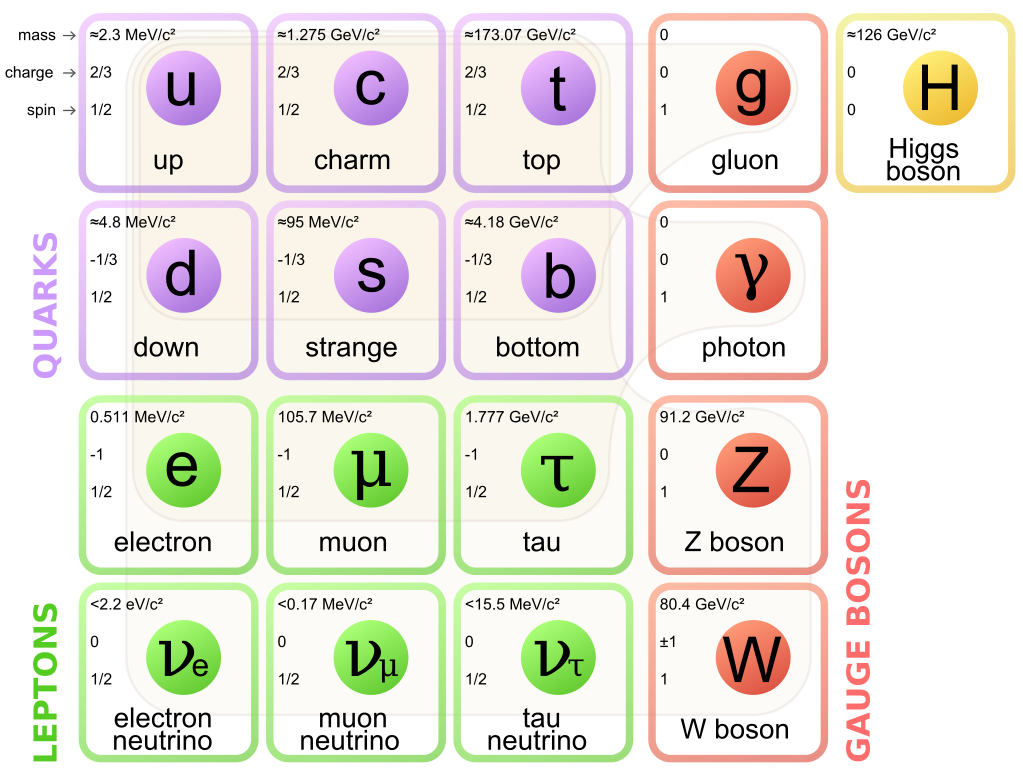
\includegraphics[width=0.75\textwidth]{theory/pics/SM_particles.png}
	\end{tabular}
	\caption{The Standard Model of elementary particles consists of  12 fundamental fermions and 4 fundamental bosons. Brown loops indicate which bosons (red) couple to which fermions (purple and green).}
	\label{fig:SM_particles}
\end{figure}

\begin{figure}[tbh!]
	\centering
	\begin{tabular}{cc}
		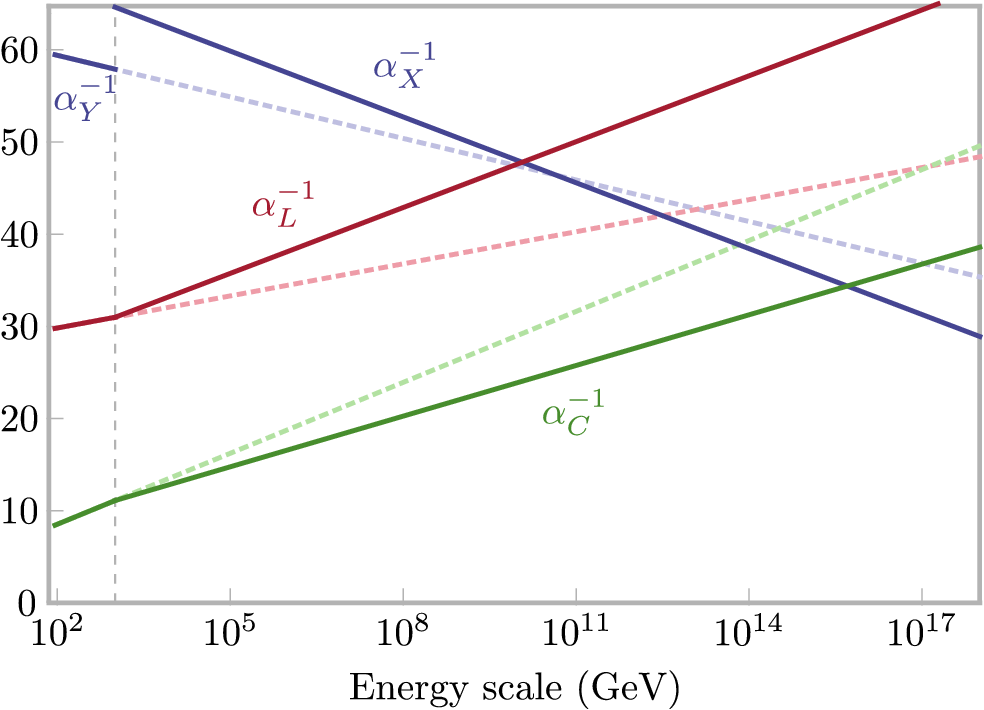
\includegraphics[width=0.75\textwidth]{theory/pics/gauge_unification.png}
	\end{tabular}
	\caption{Running of the gauge coupling constants in the SM (dashed lines) and in the model in Ref.~\cite{PhysRevD.90.013005} (solid lines). Here the $M_{331}$ scale is set to 11~TeV}
	\label{fig:gauge_unification}
\end{figure}

\clearpage

\subsection{Limitations}

\todo{Total Rework}

Although the Standard Model is very successful in describing physics at the electroweak scale, a few questions remain:

\begin{itemize}
	\item Gravity: The Standard Model does not include gravity and already for this reason alone, it cannot be a complete description of nature.
	\item No Electrostrong Unification: The hope of physics in the end is to unify all forces, but while the strong force is well represented by the SU(3), it is not unified with the other forces like it is the case for the electromagnetic and the weak force.
	\item Dark Matter: Astrophysical observations indicate a much greater accumulation of matter in the visible universe than can be explained by baryonic matter [13]. This “dark matter” cannot be explained by neutrinos, which could form only a small fraction of it. The “Modified Newtonian Dynamics” (MOND) [14] was developed in order to explain this excess within the existing theories. It was very successful, especially in explaining the measurement of galaxy rotation curves [15], until the bullet cluster [16] was discovered. Being actually two clusters passing each other, the bullet cluster shows a discrepancy between the center of the masses detected by direct observation and the center of the masses detected by gravitational lensing. This cannot be explained by MOND alone.
	\item WW Scattering: In the Standard Model, the four-vector-boson interaction becomes divergent with rising energy. If the Higgs mechanism turns out to be realized, a new term due to interactions of the vector-bosons with the Higgs is introduced, which cancels out this divergence. But this will only work, if the higgs mass is of the order of 100 GeV, and the WW scattering problem turns into the “fine-tuning” problem.
	\item Neutrino Masses: In the original Standard Model, neutrinos are set to be massless. Experiments showed that neutrinos indeed have non-zero masses [17]. In case of a sterile Dirac neutrino5, the Standard Model can be extended to include massive neutrinos. If it turns out that neutrinos are Majorana particles6, new physics beyond the Standard Model has to be introduced to explain the tiny masses of the neutrinos.
	\item Hierarchy Problem: In the Standard Model, the quantum corrections to the Higgs mass are quadratically divergent. If the Standard Model is assumed to be valid up to the Planck scale7, these corrections are huge compared to the physical Higgs mass.
\end{itemize}

\section{Supersymmetry}

Supersymmetry is one of the most intriguing and fundamental concepts in modern theoretical particle physics. It arises naturally from the combination of the two cornerstones of 20th century physics: quantum mechanics and relativity. Supersymmetry is the unique symmetry that relates the two fundamental kinds of particles: bosons, which act as the carriers of forces, and fermions, which act as the constituents of matter. Supersymmetry transformations are in a sense like the square roots of the coordinate system transformations in special relativity, and consequently supersymmetric quantum field theories have very special, improved properties, compared to ordinary relativistic quantum field theories. If supersymmetry is realized in nature, every fermion in the SM must have a bosonic partner particle and vice versa. No such superpartner particle has been observed so far but there are more and more indications that these particles might show up at the LHC experiments.


\begin{figure}[tbh!]
	\centering
	\begin{tabular}{cc}
		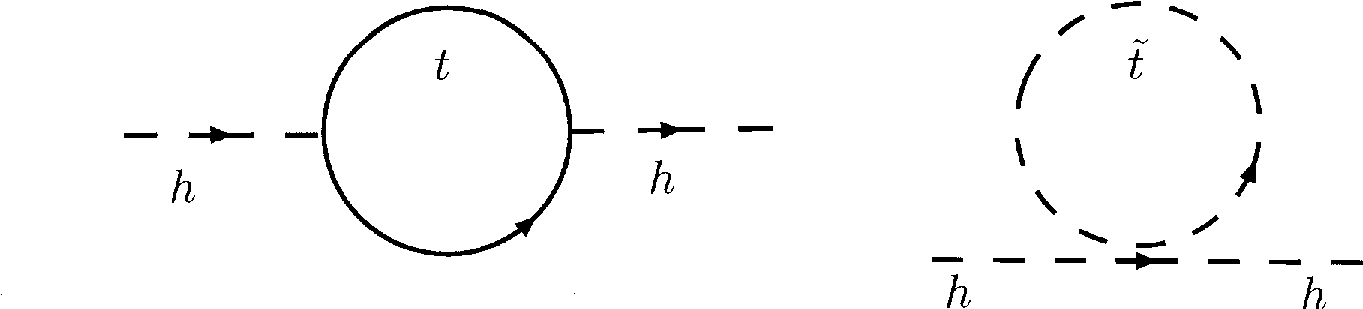
\includegraphics[width=0.75\textwidth]{theory/pics/higgs_loop.png}
	\end{tabular}
	\caption{In SUSY, the correction to Higgs mass by the top quark (L) is inherently cancelled by the contribution from the top quark's supersymmetric partner, the stop (R).}
	\label{fig:higgs_loop}
\end{figure}

\subsection{Motivations}

\subsection{The MSSM}

\begin{figure}[tbh!]
	\centering
	\begin{tabular}{cc}
		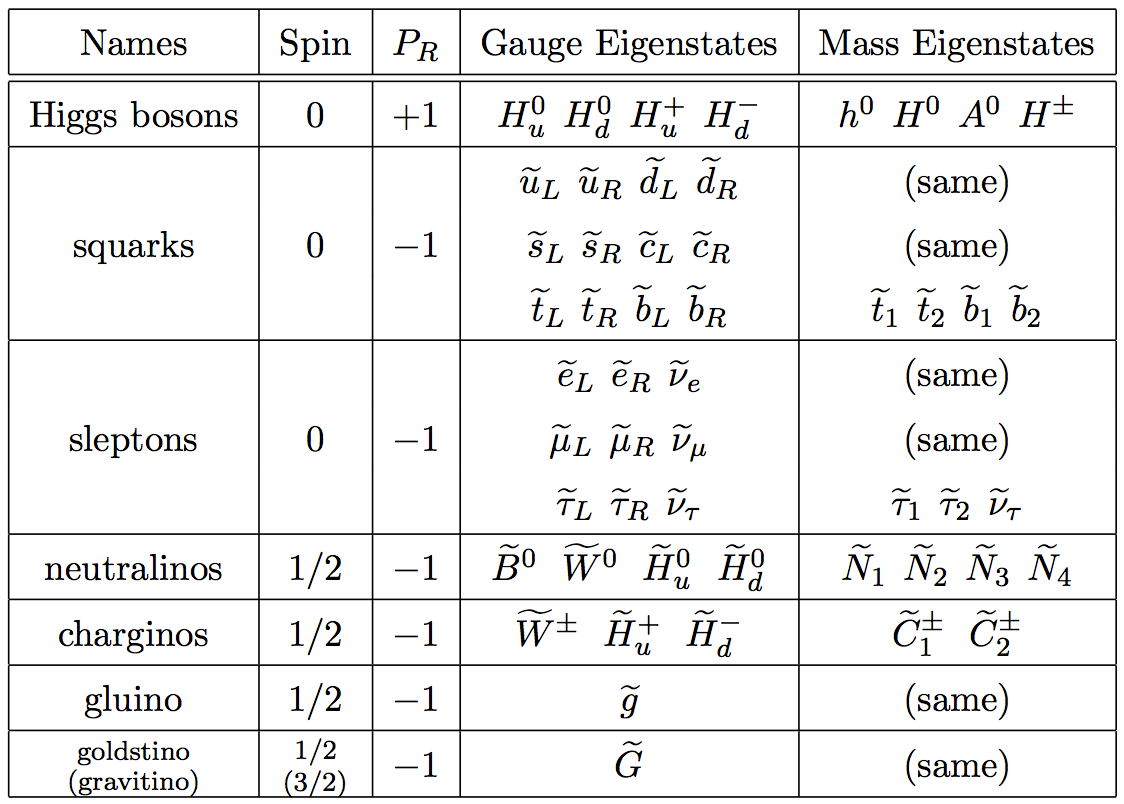
\includegraphics[width=0.75\textwidth]{theory/pics/SUSY_particles_table.png}
	\end{tabular}
	\caption{SUSY particles in MSSM~\protect\cite{Martin:1997ns}}
	\label{fig:SUSY_particles_table}
\end{figure}

\begin{figure}[tbh!]
	\centering
	\begin{tabular}{cc}
		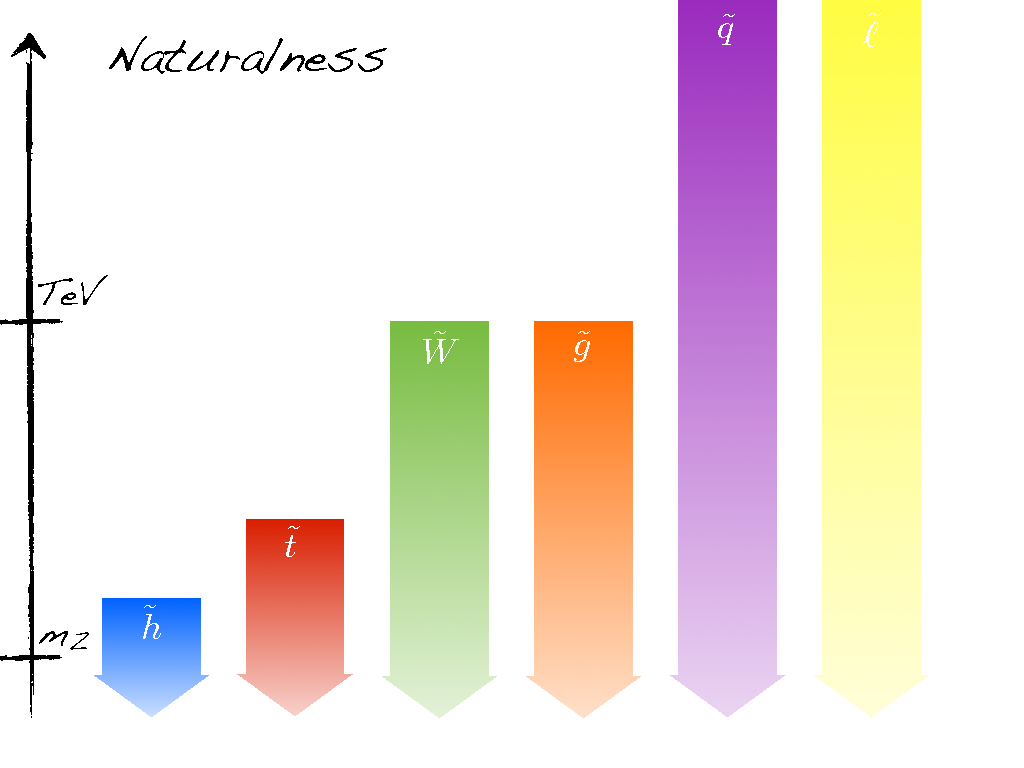
\includegraphics[width=0.75\textwidth]{theory/pics/SUSY_naturalness.png}
	\end{tabular}
	\caption{Cartoon illustration of the mass scales for various sparticles dictated solely by electroweak naturalness with sensitivity parameter $\Delta \lesssim 10$.}
	\label{fig:SUSY_naturalness}
\end{figure}




\subsection{SUSY Signatures at the LHC}
